%!TEX root = ../thesis.tex
%*******************************************************************************
%****************************** Fourth Chapter *********************************
%*******************************************************************************
\graphicspath{{Chapter4/Figs/Vector/}{Chapter4/Figs/}}

%%%%%%%%%%%%%%%%%%%%%%%%%%%%%%%%%%%%%%%%%%%%%%%%%%%%%%%%%%%%%%%%%%%%%%%%%%%%%%%%
% Trip Price Calculation System
%%%%%%%%%%%%%%%%%%%%%%%%%%%%%%%%%%%%%%%%%%%%%%%%%%%%%%%%%%%%%%%%%%%%%%%%%%%%%%%%
% - Which logic and data is required in the backend to reliably calculate a
%   trip price?
% #region
\chapter{Trip Price Calculation System}
\section{Introduction}
The term 'rule-based' in the title caters to the proposition that trip price calculations hinge on information defined as something called a rule. In this chapter, the important questions in regard to the implementation of the backend are answered, resulting in a system that deterministically calculates trip prices using rules that are restricted by user defined criteria.
% #endregion

%%%%%%%%%%%%%%%%%%%%%%%%%%%%%%%%%%%%%%%%%%%%%%%%%%%%%%%%%%%%%%%%%%%%%%%%%%%%%%%%
% The System Structure
%%%%%%%%%%%%%%%%%%%%%%%%%%%%%%%%%%%%%%%%%%%%%%%%%%%%%%%%%%%%%%%%%%%%%%%%%%%%%%%%
% #region
\section{The System Structure}
A deterministic algorithm always produces the exact same output when given a certain input. This concept is paramount in respect of a price calculation, or any financial calculation for that matter. Not only is it strange when two passengers, under the same conditions, booking the same trip, have to pay different prices. It is also impossible to guarentee the correctness of the calculation when certain parts of the computation introduce variation through side effects. This does not mean that the criteria that dictate whether rules match are not allowed to change. It does mean that given a input and a set of criteria, the resulting matched rule and price definitions, and the output should be the same every time. It may not be possible to create a completely deterministic system. Parts of the system may execute operations asynchronously, and out of order state mutations could occur, which can be contained. But there are factors that can not be controlled, such as computations of external services. These factors are side effects that are out of the scope of containment. The result of such services will be seen as the input to a deterministic function, that in contrast, should be contained. In order to reach a level of determinism, the calculation logic should manage state flawlessly. In the object-oriented programming (OOP) paradigm, state is managed through encapsulation. Object instances manage their internal state, and expose public methods to allow certain changes to be made on those instances. The functional programming (FP) paradigm treats computations as evaluations of mathematical functions. This aspect seems tailored toward the goal of reaching determinism. Using FP in conjunction with OOP, a higher order structure may be constructed using classes and encapsulation for more flexibility, while minimizing or eliminating state mutations through pure functions. In the previous chapter the second proof of concept was mentioned that separates the calculation logic from the Loopback framework as shown in Figure \ref{fig:Class Diagram}.

\begin{figure}[H]
	\centering
	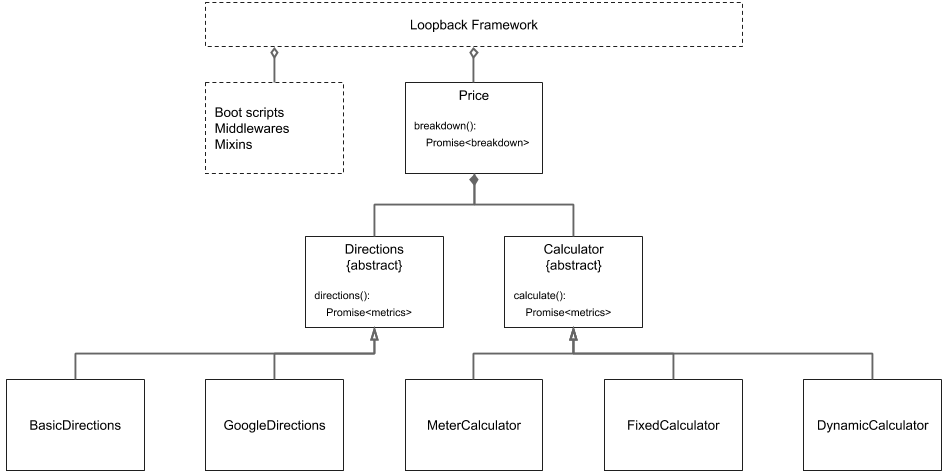
\includegraphics[width=1\textwidth]{ClassDiagram}
	\caption[Class Diagram]{High level class diagram.}
	\label{fig:Class Diagram}
\end{figure}

The isolation of the calculation and direction classes result in a more robust system, assuming that the framework is just a user of the calculation logic. The Price object is composed of a Directions and a Calculator Class, both of which expose only one method, directions and calculate respectively. The behaviour of the gathering of directions information and calculation of prices is encapsulated in different subclasses using the strategy pattern as described in \cite{gof}. Allowing behaviour to change on demand. The entities stored in the database are conceptualized in Figure \ref{fig:Data Model}, and will be referenced throughout this chapter.

\begin{figure}[H]
	\centering
	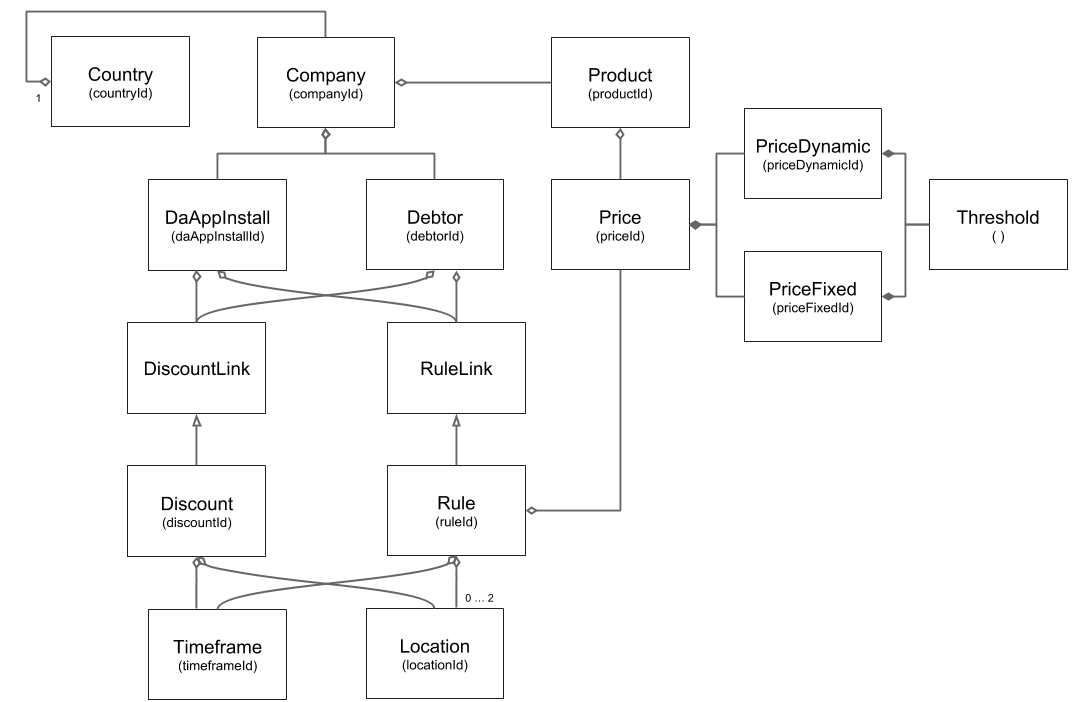
\includegraphics[width=1\textwidth]{DataModel}
	\caption[Data Model]{Conceptual data model showing database entity relations.}
	\label{fig:Data Model}
\end{figure}
% #endregion

%%%%%%%%%%%%%%%%%%%%%%%%%%%%%%%%%%%%%%%%%%%%%%%%%%%%%%%%%%%%%%%%%%%%%%%%%%%%%%%%
% The Trip Price Calculation
%%%%%%%%%%%%%%%%%%%%%%%%%%%%%%%%%%%%%%%%%%%%%%%%%%%%%%%%%%%%%%%%%%%%%%%%%%%%%%%%
% #region
\section{The Trip Price Calculation}
The process from start to end is has many edge- and corner cases. Three major stages of the process: handling the incoming request, finding the matching price rule, and calculating the prices, are explained consisely in the following subsections to provide a general overview. Important details will be expanded upon in later sections of this chapter.

\subsection{Incoming Request}
The flowchart in Figure \ref{fig:Incoming Request} shows the point where the request is received, up until the point where enough information is known to fetch rules and discounts from the database. When the request is received (1), the user is authenticated. The JSON Web Token contains the user identity, the companyId and daAppInstallId (2). The request body contains information about the ride: vehicle types, passenger count, requested date, departure, and destination.

\begin{figure}[H]
	\centering
	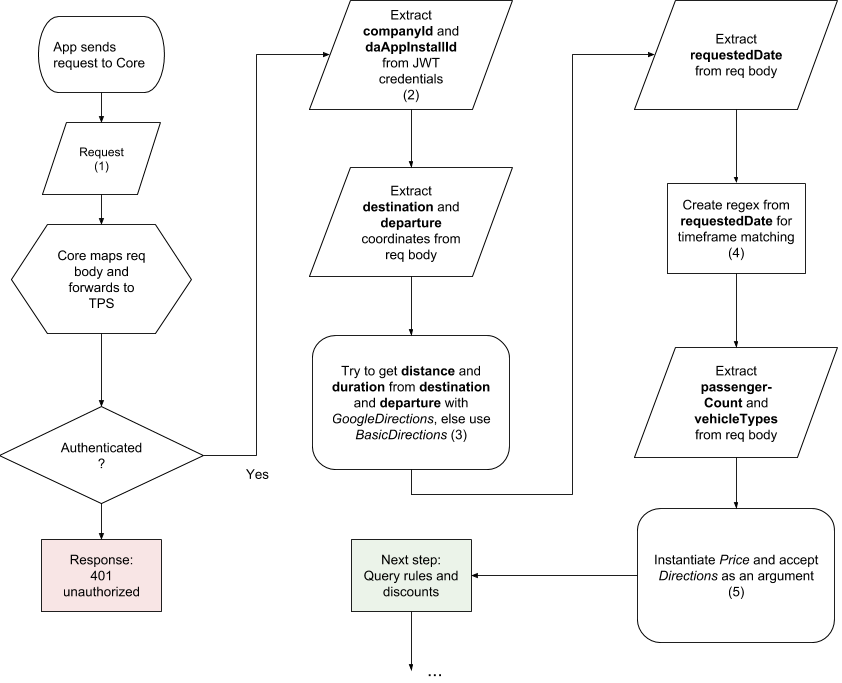
\includegraphics[width=1\textwidth]{IncomingRequest}
	\caption[Incoming Request]{The condensed flow of a trip price calculation - incoming request.}
	\label{fig:Incoming Request}
\end{figure}

The Directions class will provide an interface to retrieve trip related data. The departure and destination are fed to the Directions class, which will proceed and work out the distance and duration of the trip (3). If the GoogleDirections class is unable to determine the trip details, the BasicDirections class returns a base case result. The trip price calculation flow changes drastically when no destination or departure locations are provided in the request body. Having alternative behaviors helps dealing with providing the most accurate information possible. The strategy pattern also improves the systems resistance to change. If a different service is needed to determine the trip details in the future, it can easily take the place of one of the current services. If the trip details have not been obtained, but at least one of the two, departure or destination locations, have been provided, a database query could still work out the best matching price rule based on partial information. The requestedDate is to be converted to a regex pattern (4) for reasons explained in the timeframes section of this chapter.

\subsection{Data Aggregation}
When the user is authenticated, the system immediately requests the distance and duration of a ride by providing the departure and destination locations to the directions service. This service awaits the trip details response while it is fed to a Price class instantiation (5). The Price class will wait until matched pricing rules are provided, upon which it will perform the price calculation. Before this is the case, the aggregate queries are performed (6), trying to find a matching rule and discount for a particular company/app combination.

Two separate queries start by finding the application and company combination for which a price is calculated. If a reference to a debtor is provided, rules and discounts linked to it are used instead. The rules and discounts contain criteria in the form of timeframes and locations. A discount has basic properties while the rule has complex pricing information for products. Figure \ref{fig:Data Aggregation} shows the most important stages of the rule aggregation pipeline. The discount aggregate is a more simple version and has some of the same stages, its flowchart is therefore excluded.

\begin{figure}[H]
	\centering
	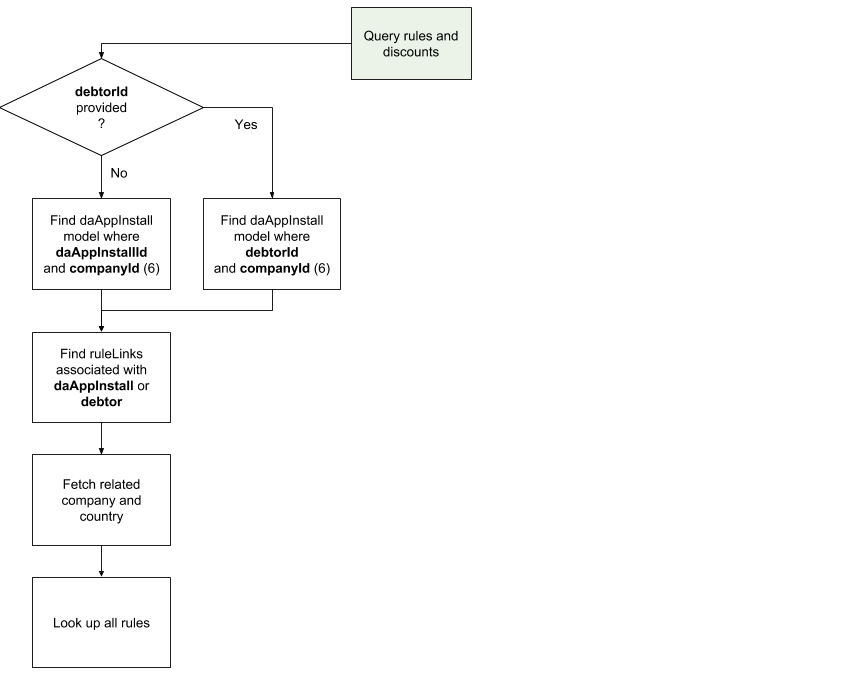
\includegraphics[width=1\textwidth]{DataAggregation}
	\caption[Data Aggregation]{The condensed flow of a trip price calculation - data aggregation.}
	\label{fig:Data Aggregation}
\end{figure}

\subsection{Calculation}
When both queries are finished, potential discounts are added to each pricing rule, which are then fed to the Price class asynchronously. A single rule has price information for each available product of that rule. If a company offers three products, it is possible to only offer two products in a given timeframe or area by associating them with a rule. For each product that is related to the price rule fetched from the database, a price breakdown is calculated. If the array of matched rules is empty, a map over the array will result in an empty array of price breakdowns. A price breakdown follows a series of logical steps, in which functions are created that have a certain default behaviour. The strategy pattern is once again applied to use the appropriate calculator for the type of calculation that is required.

% \begin{figure}[H]
% 	\centering
% 	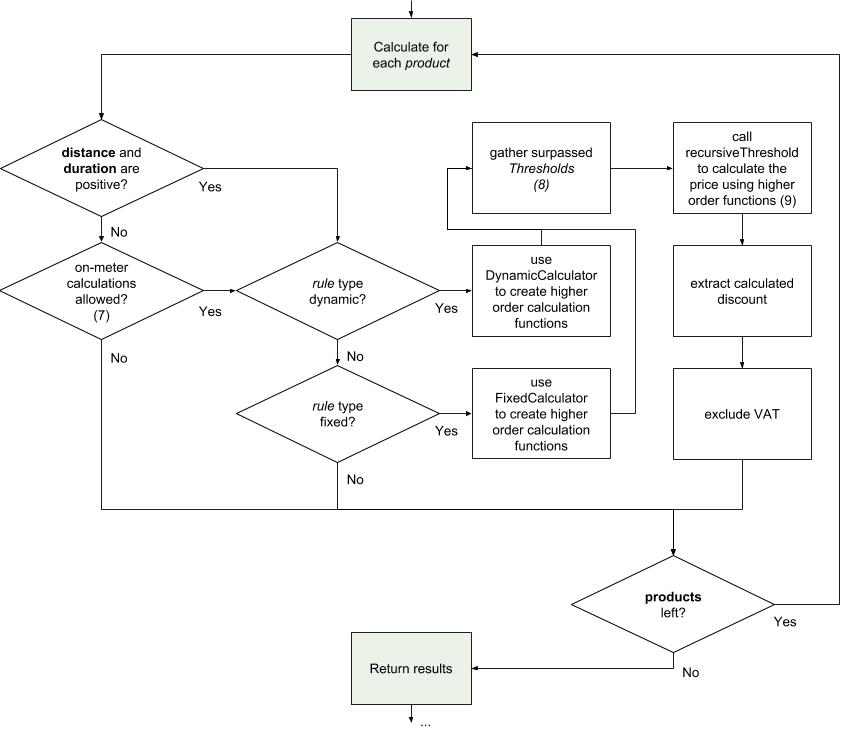
\includegraphics[width=1\textwidth]{Calculation}
% 	\caption[Calculation]{The condensed flow of a trip price calculation - calculation.}
% 	\label{fig:Calculation}
% \end{figure}

% type pricing = {
%   name: string;
%   maxPassengers: number;
%   type: vehicleType;
%   imagePath: string;
%   companyId: ObjectId;
%   company: {
%     name: string;
%     countryId: ObjectId;
%   };
%   country: {
%     name: string;
%     code: string;
%     defaultTax: number;
%     defaultCurrency: string;
%   };
%   discount?: discount;
%   prices: {
%     isEnabled: boolean;
%     isEstimated: boolean;
%     minuteWaitingPrice: number;
%     fixedPrice: number;
%     dynamicStartPrice: number;
%     dynamicMinimumPrice: number;
%     dynamicMinutePrice: number;
%     dynamicDistancePrice: number;
%     cascadingThresholdCalculation: boolean;
%     dynamicThresholds: threshold[];
%     fixedThresholds: threshold[];
%   };
%   rules: {
%     name: string;
%     type: string;
%     priority: number;
%     companyId: ObjectId;
%   };
% };


In this case, the best match is found, and price breakdowns are returned without a calculated price. This is handled by the mobile applications, as it is the case with the legacy system. But if the trip details have sucesfully been obtained, the sys
% #endregion

%%%%%%%%%%%%%%%%%%%%%%%%%%%%%%%%%%%%%%%%%%%%%%%%%%%%%%%%%%%%%%%%%%%%%%%%%%%%%%%%
% Locations
%%%%%%%%%%%%%%%%%%%%%%%%%%%%%%%%%%%%%%%%%%%%%%%%%%%%%%%%%%%%%%%%%%%%%%%%%%%%%%%%
% #region
\section{Locations}
Locations and timeframes are the big filters that reduce the amount of potential matching rules and discounts based on space and time. The implementation for location queries ...
\mynote{Working on locations}
% #endregion

%%%%%%%%%%%%%%%%%%%%%%%%%%%%%%%%%%%%%%%%%%%%%%%%%%%%%%%%%%%%%%%%%%%%%%%%%%%%%%%%
% Timeframes
%%%%%%%%%%%%%%%%%%%%%%%%%%%%%%%%%%%%%%%%%%%%%%%%%%%%%%%%%%%%%%%%%%%%%%%%%%%%%%%%
% - What was proposed as a solution to store a week schedule in a database?
% #region
\section{Timeframes}
Time plays a role in determining whether a rule has matched. The implementation of this concept should preferably offer enough freedom in the future, and should not be tailored toward one specific entity relation. Being able to reuse the timeframe entity improves maintainability of the system. The requirements state that the user must be able to define a start and end time, the days on which the times are active, and the start and end date of the timeframe. This either means that the timeframe one window of time, or that each given day has a single window of time. But if a discount should be active during night of New Years Eve, between 23h and 5h, this description would not be sufficient to cover this use case under any interpretation.

\subsection{Conventional Approach}
The legacy system takes a straight forward approach of storing time in a relational database. The begin and end of a window are stored in a record that is related to a parent timeframe entity. The timeframe has many windows that could contain a timestamp. It either finds one or many time windows that contain the timeframe. This approach covers all possibilities imaginable.

\subsection{Bitmap}
For this reason, a proposal was made to implement timeframes in a way that let users choose to describe each hour of the week, being stored as a bit map. The windows could be decreased to half an hour, resulting in twice as many bits. Three implementations have been tested, where the bitstring format offered the best outcome, as seen in \ref{appendix:slides_4}. A timeframe is stored having two ISODates (international standard: ISO 8601), and a bitstring representing the schedule for which the insert statement is shown in Listing \ref{lst:new-timeframe}.

\begin{center}
	\noindent\begin{minipage}{.45\textwidth}
		\begin{lstlisting}[caption={Improved timeframe.}, label={lst:new-timeframe}]
db.Timeframe.insert({
	startDate: new Date(2018, 4, 7),
	endDate: new Date(2019, 4, 7),
	weekSchedule:
		"001101000110011011000011
		011010110011000010111100
		101010101110100011111000
		111110011111011100100001
		101000000010111011100100
		110010000001000010101101
		010111101000000101001110"
})
\end{lstlisting}
	\end{minipage}
\end{center}

A string is a very flexible datatype. Using a regex in a query makes checking multiple bits in the string relatively easy, and enables different values next to 0 and 1. 3. A bitarray would only allow for 0 and 1 to be used. A bitstring also makes querying the data really stable, as the query will simply not match if the content of the data is not of expected length or value. Performance is not an issue if the regex column is indexed, and when prefix expressions $(/\string^/)$ are used, as per documentation in \cite{MongoDB-Regex}. As noted before, the system is easy to scale if existing data can be migrated to deal with a new amount of bits, or new character usage over bits.

\begin{lstlisting}[caption={Opening timeframe.}, label={lst:open-timeframe}]
/**
 * Date object days start at sunday, in order let monday be
 * index 0, decrease the index by one, but limit numbers
 * in the range of [0, 7).
 */
const startMonday = (d: number) => (d - 1) % 7;

/**
 * Creates a regex that spreads bits across hours of each
 * day of the week.
 */
export const regexFromDate = (date: Date) => {

	const skip =
		// Day of the week multiplied by hours a day
		startMonday(date.getDay()) * 24
		// Hour of the day
		+ date.getUTCHours();

	return { skip, timeRegex: new RegExp(`^.{${skip}}1`) };
};
\end{lstlisting}

The regexFromDate could be used to create a regex that could be used in a query to check whether a single hour within a week is set. Skip is an integer representing the number of bits that should be skipped to get to the moment represented by the date. So in order to get 11 AM - 12 AM in the presented schedule, 3 * 24 skips + 11 skip = 83 skips are to be made to find the digit 1 on thursday. Because the getDay method on JavaScript date objects return an integer resembling the day, starting at sunday, the startMonday function is used to pretend that it starts on monday.

% #endregion

%%%%%%%%%%%%%%%%%%%%%%%%%%%%%%%%%%%%%%%%%%%%%%%%%%%%%%%%%%%%%%%%%%%%%%%%%%%%%%%%
% Price Calculation Types
%%%%%%%%%%%%%%%%%%%%%%%%%%%%%%%%%%%%%%%%%%%%%%%%%%%%%%%%%%%%%%%%%%%%%%%%%%%%%%%%
% - What was proposed as a solution to store a week schedule in a database?
% #region
\section{Price Calculation Types}
Pricing information is validated before the calculation is started using the method shown in Listing \ref{lst:check-pricing-props}. The system should throw an error, as a price calculation can not proceed without the required information.

\begin{lstlisting}[caption={Find missing properties.}, label={lst:check-pricing-props}]
/**
 * Check if pricing contains valid properties and is not undefined.
 */
public static validPricingOrError(pricing: pricing | undefined): void {
	if (pricing === undefined) {
		throw new HttpError('Pricing data is undefined.');
	}
	const missing = [
		'prices',
		'rules',
		'country',
		'company',
		'type',
		'maxPassengers',
	].filter(prop => !(prop in pricing));
	if (missing.length) {
		throw new HttpError('Pricing data is missing properties:\n\t' + missing);
	}
}
\end{lstlisting}


Metrics are checked (distance duration)

Price calculator is picked depending on the rule type or if metrics are empty

\subsection{Dynamic}
The word dynamic in the dynamic price calculation means that the price can dynamically increase or decrease by a given values based on given parameters.
\subsection{Fixed}
The word fixed in the fixed price calculation means that a price is a given fixed amount under circumstances determined by the parameters.
\subsection{Meter}
The on-meter calculation simply returns a breakdown for which all values are zero. This is done by convention at taxiID, so that the mobile apps can calculate their own price based on a integrated meter inside the taxi.

% #endregion

%%%%%%%%%%%%%%%%%%%%%%%%%%%%%%%%%%%%%%%%%%%%%%%%%%%%%%%%%%%%%%%%%%%%%%%%%%%%%%%%
% Threshold Calculations
%%%%%%%%%%%%%%%%%%%%%%%%%%%%%%%%%%%%%%%%%%%%%%%%%%%%%%%%%%%%%%%%%%%%%%%%%%%%%%%%
% #region
\section{Threshold Calculations}
On top of each calculation type, prices can be defined after certain thresholds are surpassed. For example: if a taxi travels 25km, a threshold could be defined at 20km, after which the price will be 10 cents cheaper. In this case, the passenger pays a normal price for the 20 kilometers, and a cheaper price for the last 5 kilometers. The same holds for minute prices, but only for the dynamic price calculation. In the fixed price calculation, only kilometer thresholds can be defined. After a threshold is met, the fixed price will be replaced by a newly defined value. For any type of calculation, the algorithm works the same. Only the name of the metric used to measure thresholds and the actual calculation functions may change. For this reason, it is possible to define a function that recursively walks through all surpassed thresholds, then calculates a price using different calculations after each threshold was surpassed, as shown in Listing \ref{lst:threshold-recursion}

\begin{lstlisting}[caption={Recursive threshold calculation.}, label={lst:threshold-recursion}]
public static recursiveThreshold(
	thresholds: threshold[],
	calculation: Function,
	metric: number,
	cascaded: boolean = true,
): number {

	if (thresholds === undefined || thresholds.length < 1) {
		return calculation(undefined, metric);
	}

	if (!cascaded) {
		return calculation((<threshold>thresholds.shift()).value, metric);
	}

	const nextMetric = thresholds[0].threshold;
	const newMetric = metric - nextMetric;
	const price = calculation((<threshold>thresholds.shift()).value, newMetric);

	return price + Price.recursiveThreshold(
		thresholds,
		calculation,
		nextMetric,
	);
}
\end{lstlisting}

The Typescript type definitions reveal that calculation is of type Function, and thresholds is of type threshold[]. The base case returns the calculation with an undefined first argument. This forces the calculation method to use its default value, which is actually the normal kilometer or minute price. The base case will have the value of the first threshold that is met, assuring that the passenger pays the normal price up until that point. If the base case is not satisfied, the function checks whether the cascading boolean is true. This boolean determines whether each threshold should be evaluated, or only the last one. In case of the fixed price calculation, only the last threshold fixed price will be computed. But for the dynamic prices, each step has to be added to the total amount. Finally, the calculation is made using the next threshold,  and the recusive call is summed up with the calculated price. It is worth noting that even though this function is static and does not modify instance data, it is impure, leaving the passed thresholds array empty at the end.

% #endregion

%%%%%%%%%%%%%%%%%%%%%%%%%%%%%%%%%%%%%%%%%%%%%%%%%%%%%%%%%%%%%%%%%%%%%%%%%%%%%%%%
% Breakdown
%%%%%%%%%%%%%%%%%%%%%%%%%%%%%%%%%%%%%%%%%%%%%%%%%%%%%%%%%%%%%%%%%%%%%%%%%%%%%%%%
% - What should be included in the price breakdown?
% - VAT
% - Cents
% #region
\section{Breakdown}
The final result of the trip price calculation is a breakdown for every requested product. For example: if the mobile application requests prices for 'saloon' and 'limo' vehicle types, the response will at most contain an array with two breakdowns, for saloon and limo products. To ensure a seamless transition from the legacy price calculation system to TPS, the response formats should be identical. Still an improvement, if profitable enough, could be taken into consideration. One requirement of the price breakdown states that the tax should be included, but as shown in Listing \ref{lst:legacy-breakdown} the included tax is part of the breakdown. Is it by mistake or design?

\begin{lstlisting}[caption={Legacy price breakdown}, label={lst:legacy-breakdown}]
[
	{
		"vehicleType": "saloon",
		"maxPassengers": "4",
		"price": {
			"currency": "EUR",
			"total": 850,
			"breakdown": {
				"route": 802,
				"tax": 48,
				"toll": 0,
				"parking": 0,
				"waiting": 0,
				"discount": 0
			}
		},
		"fixedPrice": "true"
	}
]
\end{lstlisting}

Two possible solutions were proposed having VAT included in the price. The first solution extracts the tax element from the breakdown, so that the sum of the breakdown would add up to the total price where VAT is included in the price as shown in Listing \ref{lst:new-breakdown}. As demonstrated in Appendix \ref{appendix:slides_2_breakdown}, a breakdown is easily constructed in four steps when VAT is included.

\begin{lstlisting}[caption={Improved price breakdown}, label={lst:new-breakdown}]
[
	{
		"vehicleType": "estate",
		"maxPassengers": 4,
		"isEstimated": false,
		"price": {
			"breakdown": {
				"route": 8300,
				"toll": 0,
				"parking": 0,
				"waiting": 0,
				"discount": -1650
			},
			"currency": "EUR",
			"total": 6650,
			"tax": {
				"amount": 400,
				"percentage": 6
			}
		}
	},
	...
]
\end{lstlisting}

Keep in mind that unlike the listings the prices in the proposal are not displayed in cents. The second solution maintains the legacy format, but has to recalculate the prices without VAT. This could have downsides unlike the first approach:

\begin{enumerate}
	\item If an error is detected in the calculation, it is hard to trace back which components contributed to the total VAT. This would be even harder when each component uses its own VAT percentage.
	\item It takes extra steps to calculate the price of each component excluding VAT.
	\item Rounding the individual components could result in a sum that is not equal to the total displayed in the breakdown.
\end{enumerate}

The first proposal is chosen to be implemented, where the flag 'fixedPrice' is replaced by the 'isEstimated' flag to clearly reflect its purpose.
% #endregion

%%%%%%%%%%%%%%%%%%%%%%%%%%%%%%%%%%%%%%%%%%%%%%%%%%%%%%%%%%%%%%%%%%%%%%%%%%%%%%%%
% Testing
%%%%%%%%%%%%%%%%%%%%%%%%%%%%%%%%%%%%%%%%%%%%%%%%%%%%%%%%%%%%%%%%%%%%%%%%%%%%%%%%
%
\section{Determinism}
- Database query return same result
- Classes and project structure operate in the same way each time
- Side effects like google maps reduced by enlarging points locations
- FP pure functions programming styles
- tests
- CI CD
- interfaces
- static strong types
- type hinting
- OOP en FP mixen
- OOP voor grote structuur
- FP voor solide operaties
- SOLID
- Gang of Four
- Loose coupling high cohesion
- Async
- Strategy pattern

Unit tests are to be written to cover the most important aspects of the system. New features often introduce bugs by adding functionalities that are broken, although the reliability of the existing functionalities may also be impacted because of changes in the existing code. To prevent units of code from malfunctioning, regression tests may be implemented to validate whether a unit still functions according to a set of conditions. Static and dynamic tests may be performed using the framework Mocha \cite{mocha} and the assertion library Chai \cite{chai}. To further reduce the chances of introducing bugs, some additional techniques could be used, including Software Validation techniques. Linting is the process of running a program that will analyse code for potential errors. Static analysis tools may be used to find code smells. Continuous Integration may be implemented to ensure that valid builds are deployed. A comparison was made in Appendix \ref{appendix:pregame}, chapter 4.9, between CI tools. Various CI tools were implemented in previously mentioned proofs of concept.

State and mutations should be fully encapsulated, leaving only static functions exposed. These functions aim to mutate data in a pure way, meaning that no state is changed outside of the function scope, and that the function is absolutely honest about its parameters and return values. As discussed in the previous chapter, Typescript plays an important role in mixing OOP and FP together. The database schema desgin as shown in the previous chapter gives an inpression on the different pieces of information required to calculate a price. Such a schema provides a good insight in the relationships that different entities have, but may distract from the actual story that is happening within each calculation.

The object-oriented programming (OOP) paradigm offers many ways to keep a system structured. Good software design has low coupling and high cohesion, meaning that software components should have a high degree of belongingness, and a low degree of dependence in respect of eachother. As stated in the previous chapter, another paradigm that could potentially improve the price calculation system is called: functional programming (FP).

% #endregion

%%%%%%%%%%%%%%%%%%%%%%%%%%%%%%%%%%%%%%%%%%%%%%%%%%%%%%%%%%%%%%%%%%%%%%%%%%%%%%%%
% Premise
%%%%%%%%%%%%%%%%%%%%%%%%%%%%%%%%%%%%%%%%%%%%%%%%%%%%%%%%%%%%%%%%%%%%%%%%%%%%%%%%
% #region
\section{Premise}
\[\textit{Which logic and data is required in the backend to reliably calculate a trip price?}\]\hfill

\mynote{Conclusion for chapter 4}
% How can determinism of price computations be guarenteed?
% Which criteria determine whether rules match?
% In what way can the three original pricing rule types be implemented? (fixed, dynamic, and threshold prices)